
%%%%%%%%%%%%%%%%%%%%%%%%%%%%%%%%%%%%%%%%%%%%%%%%%%%%%%%%%%%%%
%%%%%%%%%%%%%%%%%%%%%%%%%%%%%%%%%%%%%%%%%%%%%%%%%%%%%%%%%%%%%
%
%  %%%%%%%  %    %  %%%%%%  %%%%%%  %%%%%%%  %%%%%%%  %%%%%
%  %        %    %  %    %  %     %    %     %        %    %
%  %        %    %  %%%%%%  %     %    %     %        %    %
%  %        %%%%%%  %    %  %%%%%%     %     %%%%%    %%%%%
%  %        %    %  %    %  %          %     %        %    %
%  %%%%%%%  %    %  %    %  %          %     %%%%%%%  %     %
%
%%%%%%%%%%%%%%%%%%%%%%%%%%%%%%%%%%%%%%%%%%%%%%%%%%%%%%%%%%%%%
%%%%%%%%%%%%%%%%%%%%%%%%%%%%%%%%%%%%%%%%%%%%%%%%%%%%%%%%%%%%%

\chapter{Network Coding and Routing Sheaves}
\label{sec:nc_coding}

In the previous section, we introduced the language of barcodes and integrated them with a cosheaf-theoretic perspective on Morse theory and persistent homology. The fundamental idea was that by decomposing a cosheaf into indecomposables, we were able to understand cosheaf homology via the Borel-Moore homology of the barcode. In this section, we attempt to do the same thing for cellular sheaves on graphs. We apply the barcode perspective, wherever possible, to a class of sheaves introduced by Robert Ghrist and Yasuaki Hiraoka~\cite{GH-ncs}. These sheaves were specifically designed to model the flow of information over graphs and the generalized barcode decomposition can aid in visualizing this flow. 

First, we review some basic definitions for graphs.

\begin{defn}\index{quiver}\index{graph}
	Let $X$ be a directed graph consists of a pair of sets $E$ and $V$ of edges and vertices and a pair of functions $h,t:E\to V$ that return the \textbf{head} and \textbf{tail} of an edge respectively. A directed edge goes from its tail to its head. The set of \textbf{incoming edges} to a vertex $v$, written $in(v)$, is the set of edges whose heads are $v$, i.e. $h^{-1}(v)$. The set of \textbf{outgoing edges} at $v$ is the set of edges whose tails are at $v$, i.e. $t^{-1}(v)=v$.
\end{defn}

\begin{defn}\index{capacity}
	Let $X$ be a directed graph with vertex set $V$ and edge set $E$. A \textbf{capacity function} is a function $c$ from the edge set to either the non-negative reals $\RR_{\geq 0}$ or the non-negative integers $\ZZ_{\geq 0}$.
\end{defn}

\begin{defn}[Network Coding Cell Sheaf]\index{network coding sheaf}\index{sheaf!network coding}
	Suppose $X$ is a directed graph with a capacity function $c$. A \textbf{network coding sheaf} on $X$ is a cellular sheaf $F:X\to\Vect$ constructed as follows: 
	\begin{itemize}
		\item To an edge $e\in X$ we let $F(e)=k^{c(e)}$, a vector space of dimension equal to the capacity.
		\item To a vertex $v$ we let $F(v)=k^{c(v)}\cong \oplus_{e_i\in in(v)} k^{c(e)}$.
		\item The restriction maps are given by ordinary projections for the incoming edges, i.e. $\rho_{e_i,v}:=proj_{F(e_i)}$ for $e_i\in in(v)$, but for the outgoing edges some non-trivial coding may be performed, i.e. any linear map $\Phi_{e_k,v}:F(v)\to F(e_k)$ for $e_k\in out(v)$ will do. We write $\Phi_v=\oplus_{e_k\in out(v)} \Phi_{v,e_k}$ for the \textbf{total coding} through $v$.
	\end{itemize}
\end{defn}

\begin{rmk}
	It should be noted that in~\cite{GH-ncs}, they do not use cellular sheaves. This was primarily due to the lack of a good reference.
\end{rmk}

\begin{figure}[ht]
\centering
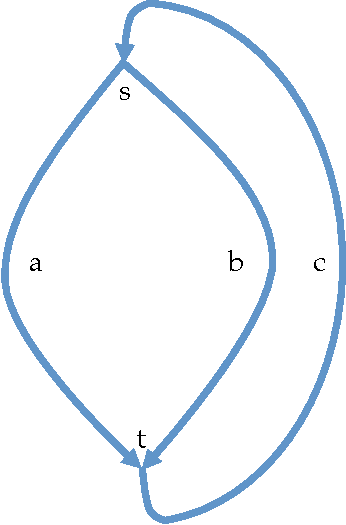
\includegraphics[width=.5\textwidth]{nc_graph_dir.pdf}
\caption{Graph with Decoding Wire}
\label{fig:nc_graph_dir}
\end{figure}

In~\cite{GH-ncs} they do not define network coding sheaves for arbitrary directed graphs. Instead, they consider a graph with a distinguished set of sources and targets (senders and receivers) and they augment the graph by adding \textbf{decoding wires} directed to go from a target vertex back to a subset of source vertices. Heuristically for Ghrist and Hiraoka, the purpose of these edges is to make global sections of this sheaf correspond to closed loops through the graph. This topological reasoning is correct, but oversimplifies how network codings can produce counterintuitive weavings and splittings of data.

\begin{ex}
	Consider the graph in Figure~\ref{fig:nc_graph_dir} with constant capacity function $c = 1$. Consequently, all edges and vertices get a one dimensional vector space $k=\RR$ with the exception of $F(t)\cong k^2$. Define the coding maps $\rho_{a,s}=\id=\rho_{b,s}$ and
	\[
		\rho_{c,t}=\begin{bmatrix} \frac{1}{2} & \frac{1}{2}\end{bmatrix}.
	\]
	We pick a local orientation implied by the source and target vertices. The one and only coboundary matrix can be written as follows:
	\[
		\delta^0:=\begin{bmatrix}
				-1 & 1 & 0 \\
				-1 & 0 & 1 \\
				1 & -1/2 & -1/2
		\end{bmatrix}
	\]
	Consequently, $H^0(X;F)\cong H^1(X;F)\cong k$. The one global section is supported over the entire graph; it is not simply a loop through the graph.
\end{ex}

The previous example of a network coding sheaf is an example of an indecomposable sheaf that is not a generalized barcode in the sense of Definition~\ref{defn:generalized_bc}. To better understand the flow of data over graphs, as well as the utility of the barcode perspective, we consider a simpler class of network coding sheaves.

\section{Duality and Routing Sheaves}

\begin{defn}[Routing Sheaf]\index{routing sheaf}\index{sheaf!routing}
	A particular type of network coding sheaf is a \textbf{routing sheaf}. Here we assume that the capacity function is constant $c = 1$, and the coding maps $\Phi_v$ can be written as a binary matrix with at most one $1$ in each column and row. Said another way, at a vertex $v$ the total coding map maps to zero as many incoming edges as desired, so long as there is a bijection of the remaining incoming edges and a subset of the outgoing edges. The total coding map through $v$ is then a matrix representation of this bijection.
\end{defn}

The advantage of routing sheaves is that they are simple to visualize: Start at a source and use a color pen to track how an edge emanating from that source gets bounced around under the routing directions at each subsequent vertex. If at any point in your drawing you run into a vertex that sends your edge's data to zero, stop on that vertex with your pen. This argument essentially establishes the following proposition. 

\begin{prop}[Structure Theorem for Routing Sheaves]\label{prop:rout_bc}
	Suppose $X=(V,E,h,t)$ is a directed graph, then every routing sheaf $F:X\to\Vect$ can be realized as the pushforward with compact support of a disjoint union of half-open intervals $[\textrm{---}[$ or circles, whose images can intersect only at vertices.
\end{prop}

A consequence of this result combined with Poincar\'e duality is the following corollary.

\begin{cor}[Duality]\index{duality!for routing sheaves}\index{routing sheaf!duality}
	For any routing sheaf $F$ one has
	\[
		H^0(X;F)\cong H^1(X;F).
	\]
\end{cor}
\begin{proof}
	By Proposition~\ref{prop:rout_bc}, every network coding sheaf can be written as a direct sum of constant sheaves supported on half-open intervals or circles. Half-open intervals embedded into compact spaces (extending by zero using $j_!$) have trivial cohomology in both degrees. Poincar\'e duality for $S^1$ establishes the corollary.
\end{proof}

One can also prove this duality in the more general setting of network coding sheaves via a simple combinatorial argument.

\begin{prop}
	For an any network coding sheaf $F$, we have the following isomorphisms:
	\[
		\bigoplus_v F(v) \cong \bigoplus_e F(e) \qquad  H^0(X;F)\cong H^1(X;F)
	\]
\end{prop}
\begin{proof}\index{duality!network coding sheaf}\index{network coding sheaf!duality}
	By construction of a network coding sheaf there is a bijection between the sum of the vector spaces over the edges $e\in in(v)$ and the vector space over the vertex $v$.
	\[
		\bigoplus_{e\in in(v)} F(e) = F(v).
	\]
	By definition of a graph, every edge is the incoming edge for a unique vertex. Thus, by summing over all vertices, we sum over all edges without double-counting. This proves the first isomorphism. The second isomorphism follows by the rank-nullity theorem.  
\end{proof}

Ideally, one could interpret these cohomology groups as something meaningful to obtain a useful duality result, but this is still missing. Ghrist and Hiraoka interpret $H^0$ as a vector space spanned by independent information flows, but in the case of routing sheaves, $H^1$ is the group that counts closed trajectories of information flow. For routing sheaves, one could say that the Poincar\'e dual of the fundamental class of an information loop would yield a point whose removal would cease the flow of information. One might call this a ``cut equals flow'' theorem. This is only a pale shade of the greater ``Max-Cut Min-Flow'' theorem~\cite{efs-mfmc, ff-mfmc, seymour-matroids}, which compares the maximum possible flow with the minimum capacity cut required to disconnect the graph.

\section{Counting Paths Cohomologically, or Failures thereof}

Regardless of network coding sheaves connections with duality, one would like to know what information cellular sheaf cohomology can capture over a graph. Is it possible, for example, to build a sheaf that encodes source-to-target paths cohomologically? Suppose we allow the source to have its own independent capacity, without regard for the number of incoming edges. As the next example shows such a ``pseudo network coding'' (NC) sheaf cannot encode source-to-target paths cohomologically.

\begin{figure}[!ht]
\begin{minipage}[b]{0.47\linewidth}
\centering
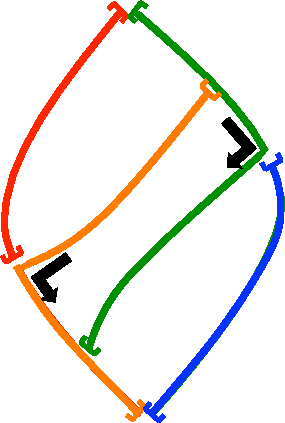
\includegraphics[scale=1]{ncs_no_decode.pdf}
\caption{No Decoding Edge}
\label{fig:ncs_no_decode}
\end{minipage}
\hfill
\begin{minipage}[b]{0.47\linewidth}
\centering
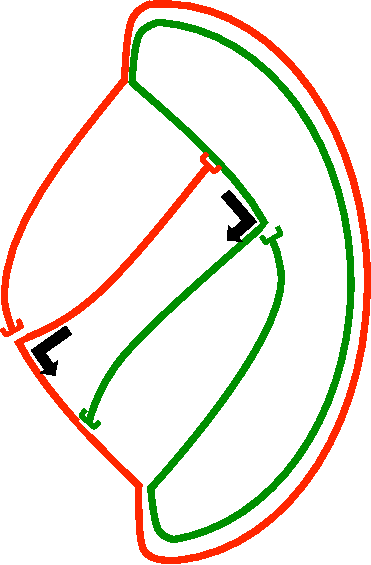
\includegraphics[scale=1]{ncs_decode.pdf}
\caption{Decoding Edge}
\label{fig:ncs_decode}
\end{minipage}
\end{figure}

\begin{ex}[Decoding Edge and Barcodes]\index{decoding edge}
In Figures~\ref{fig:ncs_no_decode} and~\ref{fig:ncs_decode}, the barcode decomposition of a network coding sheaf is drawn with and without a decoding edge.
With the particular choices made there is no flow from source to target. Yet the sheaf in Figure~\ref{fig:ncs_no_decode} decomposes as the constant sheaf on two half open intervals and two closed intervals:
\[
F_{no}\cong (j_o)_! k_{[0,1)}\oplus(j_b)_! k_{[0,1)}\oplus (i_r)_* k_{[0,1]}\oplus (i_g)_*k_{[0,1]} \Rightarrow H^0(X;F_{no})\cong k^2.
\]
This is bad if we want our sheaf to encode cohomologically the presence of source-to-target information paths.

However, with the use of a decoding edge (decoding edges) the network decomposes into only two half open intervals:
\[
F_{de}\cong (j_r)_!k_{[0,1)}\oplus(j_g)_!S k_{[0,1)} \Rightarrow H^0(X;F_{de})\cong 0
\]
which was wanted.
\end{ex}

\section{Network Coding Sheaf Homology}
\label{subsubsec:sheaf_homology_graphs}
\index{sheaf!homology, cellular!examples}
One of the virtues of the network coding sheaves is that they are easy to construct, have interesting sheaf cohomology, and provide lots of examples. As such, we will use them as a testing ground for the new theory of sheaf homology developed in Section~\ref{subsec:sheaf_homology}.

\begin{figure}[ht]
\centering
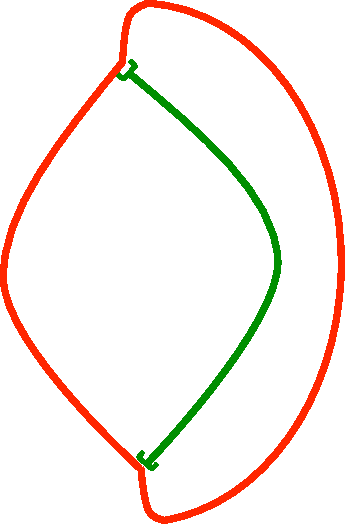
\includegraphics[width=.5\textwidth]{nc_1.pdf}
\caption{Network Coding Sheaf}
\label{fig:nc_1}
\end{figure}

\begin{ex}
Consider the network coding sheaf implied by Figure~\ref{fig:nc_1}. Viewed as a diagram of vector spaces, it takes the following form:
\[
\xymatrix{ & \ar[ld]^1 k_s \ar[rd]_0 \ar[rrd] & & \\
		k_a & & k_b & k_c \\
		& k_t^2 \ar[ul]_{\pi_1} \ar[ur]^{\pi_2} \ar[urr]_{\pi_1} & & }
\]
Since the category of complexes of sheaves is additive, we can consider each indecomposable sheaf separately and compute its sheaf homology. If one considers just the red loop as a constant sheaf (barcode) $R$, it takes the following form:
\[
\xymatrix{ & \ar[ld]^1 k_s \ar[rd] \ar[rrd] & & \\
	k_a & & 0 & k_c \\
        & k_t \ar[ul]_{1} \ar[ur]^{} \ar[urr]_{1} & & }
\]
A projective sheaf that surjects onto $R$ is supported on the star of $s$ and $t$ respectively, i.e. $P_0:=\{s\}\oplus\{t\}$:
\[
\xymatrix{ & \ar[ld]^1 k_s \ar[rd] \ar[rrd] & & \\
	k_s\oplus k_t & & k_s\oplus k_t & k_s\oplus k_t \\
        & k_t \ar[ul]_{1} \ar[ur]^{} \ar[urr]_{1} & & }
\]
The kernel sheaf of the natural transformation $P_0\Rightarrow R$ is also projective, which we call $P_1$ and finishes the projective replacement of the sheaf $R$.
\[
\xymatrix{ & 0 \ar[ld] \ar[rd] \ar[rrd] & & \\
	[1\, -1] & & k_s\oplus k_t & [1\, -1] \\
        & 0 \ar[ul] \ar[ur]^{} \ar[urr] & & }
\]
If we take the colimit of $P_1$ and $P_0$ separately, the sheaf map $P_1\to P_0$ induces a map on colimits that defines the boundary in the chain complex computing sheaf homology:
\[
\partial_1: k^4\to k^2 \qquad 
\begin{bmatrix} 1 & 1 & 0 & 1 \\
-1 & 0 & 1 & -1\end{bmatrix}
\quad \Rightarrow \quad H_0(X;R)=0 \quad H_1(X;R)\cong k^2
\]
 Repeating the same reasoning for the green barcode $G$ yields homology groups $H_0(X;G)=0$ and $H_1(X;G)\cong k$. Since our original network coding sheaf $F$ is a direct sum $R\oplus G$ we obtain that the sheaf homology of the sheaf in Figure~\ref{fig:nc_1} is
\[
H_0(X;F)=0 \qquad H_1(X;F)\cong k^3.
\]
\end{ex}

\begin{figure}[ht]
\centering
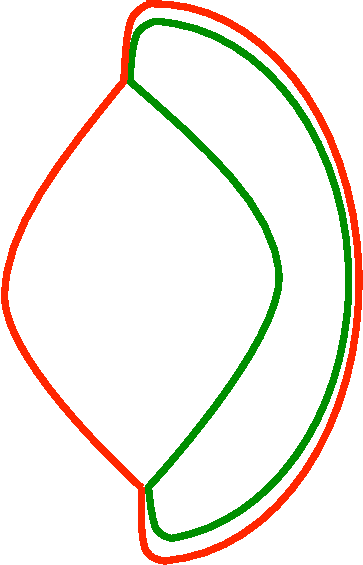
\includegraphics[width=.5\textwidth]{nc_2.pdf}
\caption{Network Coding Sheaf with Two Decoding Wires}
\label{fig:nc_2}
\end{figure}

\begin{exr}
As an exercise, and to indicate the sensitivity of sheaf homology to its embedding, we ask the reader to verify that the sheaf homology groups of the sheaf in Figure~\ref{fig:nc_2} are
\[
H_0(X;F)=0 \qquad H_1(X;F)\cong k^8.
\]
\end{exr}
